
\chapter{Коэффициенты ветвления и обобщенная резольвента Бернштейна-Гельфанда-Гельфанда}
\label{cha:BGG}

Как мы показали в предыдущей главе, рекуррентные соотношения для коэффициентов ветвления основываются на определенном разложении сингулярного элемента. В данной главе мы показываем, что такое разложение может использоваться для построения параболических модулей Верма и получения обобщенных формул Вейля-Верма для характеров. Также мы демонстрируем, что ветвление для произвольной редуктивной подалгебры связано с БГГ резольвентой и демонстрирует свойства резольвенты в категории $\mathcal{O}^{p}$ \cite{lepowsky1977generalization} (параболического обобщения категории $\mathcal{O}$ \cite{bernstein1976category}).

Резольвента для неприводимых модулей в терминах бесконечномерных модулей важна для теории интегрируемых спиновых цепочек \cite{derk1008}. В подходе  $\mathcal{Q}$-оператора Бакстера \cite{derk09} общие трансфер-матрицы, соответствующие (обобщенным) модулям Верма, факторизуются в произведение операторов Бакстера. Резольвента позволяет вычислить трансфер-матрицы для конечномерных вспомогательных пространств.

Чтобы продемонстрировать связь БГГ резольвенты с ветвлением мы используем рекурсивный подход, представленный в работе \cite
{2010arXiv1007.0318L} (аналогичный подход для максимальных вложений использовался в работе \cite{ilyin812pbc}) и изложенный в главе \ref{cha:affine-lie-algebras}. Мы рассматриваем подалгебру $\af \hookrightarrow \gf$ вместе с $\afb$ -- ``ортогональным партнером'' $\af$ по отношению к форме Киллинга, а также подалгебру $\widetilde{\afb}:=\afb\oplus \frak{h}_{\perp }$, где $\frak{h}=\frak{\frak{h}_{\af}}\oplus
\frak{h}_{\afb}\oplus \frak{h}_{\perp }$. Для любой редуктивной подалгебры $\af$ алгебра $\afb\hookrightarrow \gf$ регулярна и редуктивна. Для интегрируемого модуля старшего веса $%
L^{\left(\mu \right) }$ и ортогональной подалгебры  $\af_{\bot }$ мы рассматриваем сингулярный элемент $\Psi ^{\left( \mu \right) }$ (числитель в формуле Вейля для характеров $ch\left( L^{\mu }\right) =\frac{\Psi ^{\left(
\mu \right) }}{\Psi ^{\left( 0\right) }}$, см., например,  \cite
{humphreys1997introduction}) и знаменатель Вейля $\Psi _{\af_{\bot
  }}^{\left( 0\right) }$ для ортогонального партнера. Ниже мы показываем, что элемент  $\Psi _{\gf%
}^{\left( \mu \right) }$ может быть разложен в комбинацию числителей Вейля $\Psi _{\af_{\bot }}^{\left( \nu \right) }$, где $\nu \in P_{%
\mathfrak{a}_{\bot}}^{+}$. Это разложение дает возможность построить множество модулей старшего веса $L_{\afb}%
^{\mu _{\afb}}$. В том случае, если вложение\ $\af%
_{\bot }\hookrightarrow \gf$ \ удовлетворяет ``стандартным параболическим'' условиям, эти модули порождают параболические модули Верма $M_{\left(
\afb \hookrightarrow \gf\right) }^{\mu _{%
\afb}}$, так что исходный характер $ch\left(
L^{\mu }\right) $ в итоге раскладывается в знакопеременную сумму таких модулей. С другой стороны, если параболическое условие нарушено, конструкция сохраняется и порождает разложение по отношению к набору обобщенных модулей Верма  $M_{\left( \widetilde{\frak{b}_{\perp }},\gf\right) }^{\mu _{%
\widetilde{\afb}}}$, где $%
\widetilde{\frak{b}_{\perp }}$ уже не является подалгеброй в $\gf$, а оказывается сжатием $\widetilde{\afb}$.

Некоторые общие свойства предложенного разложения формулируются в терминах  формального элемента $\Gamma _{\af\rightarrow \gf}$, называемого ``веером вложения''. Использование этого инструмента позволило сформулировать простой и явный алгоритм для вычисления правил ветвления, подходящий для произвольной (максимальной или не максимальной) подалгебры в аффинной алгебре Ли \cite{2010arXiv1007.0318L}.

Возможные обобщения полученных результатов обсуждаются в Разделе \ref{sec:conclusions}.

\section{Ортогональная подалгебра и сингулярные элементы}

\label{sec:recurr-form-branch}

В этом разделе мы покажем, как рекуррентный подход к проблеме ветвления естественным образом приводит к представлению формального характера $\frak{g}$-модуля в виде комбинации характеров, соответствующих параболическим (обобщенным) модулям Верма. Рассмотрим редуктивную алгебру Ли  $\frak{g}$ и ее редуктивную подалгебру $\frak{a}\subset \frak{g}$.
Пусть  $L^{\mu} $ -- интегрируемый модуль старшего веса алгебры  $\frak{g}$, $\mu \in P^{+}$.  Будем считать  $L^{\mu}$ вполне приводимым по отношению к подалгебре $\frak{a}$,
\begin{equation*}
L_{\frak{g}\downarrow \frak{a}}^{\mu }=\bigoplus\limits_{\nu \in P_{\frak{a}%
}^{+}}b_{\nu }^{\left( \mu \right) }L_{\frak{a}}^{\nu }.
\end{equation*}
Это разложение может быть записано в терминах формальных характеров с использованием оператора проекции  $\pi _{\frak{a}}$ (на весовое пространство $\frak{h_{a}}^{\ast }$):
\begin{equation}
\pi _{\frak{a}}ch\left( L^{\mu }\right) =\sum_{\nu \in P_{\frak{a}%
}^{+}}b_{\nu }^{(\mu )}ch\left( L_{\frak{a}}^{\nu }\right) .
\label{branching1}
\end{equation}
Для модуля  $L^{\mu }$ существует БГГ резольвента (см. \cite
{bernstein1976category,bernstein1975differential,bernstein1971structure} и
\cite{humphreys2008representations}). Все члены фильтрующей последовательности представляются суммами модулей Верма со старшими весами $\nu$, сильно связанными с $\mu$:
\begin{equation*}
\left\{ \nu \right\} =\left\{ w\left( \mu +\rho \right) -\rho |w\in
W\right\} .
\end{equation*}

\subsection{Ортогональная подалгебра}

Пусть  $\frak{h}_{\frak{a}}$ -- подалгебра Картана в  $\mathfrak{g}$. Для  $\mathfrak{a}\hookrightarrow \frak{g}$ введем ``ортогонального партнера''  $\mathfrak{a}_{\bot }\hookrightarrow \frak{g}$.

Рассмотрим корневое подпространство  $\frak{h}_{\perp \frak{a}}^{\ast }$, ортогональное к $\frak{a}$,
\begin{equation*}
\frak{h}_{\perp \frak{a}}^{\ast }:=\left\{ \eta \in \frak{h}^{\ast }|\forall
h\in \frak{h}_{\frak{a}};\eta \left( h\right) =0\right\} ,
\end{equation*}
и корни  $\frak{g}$ (соответственно, положительные корни),  ортогональные к $\frak{a}$,
\begin{eqnarray}
\Delta _{\frak{a}_{\perp }} &:&=\left\{ \beta \in \Delta _{\frak{g}}|\forall
h\in \frak{h}_{\frak{a}};\beta \left( h\right) =0\right\} ,
\label{delta a ort} \\
\Delta _{\frak{a}_{\perp }}^{+} &:&=\left\{ \beta ^{+}\in \Delta _{\frak{g}%
}^{+}|\forall h\in \frak{h}_{\frak{a}};\beta ^{+}\left( h\right) =0\right\} .
\notag
\end{eqnarray}
Обозначим символом  $W_{\frak{a}_{\perp }}$ подгруппу  $W$, порожденную отражениями  $w_{\beta }$ с корнями  $\beta \in \Delta_{\frak{a}_{\perp}}^{+}$. Корневая подсистема  $\Delta _{\frak{a}_{\perp }}$ определяет подалгебру  $\frak{a}_{\perp }$, имеющую подалгебру Картана $\frak{h}_{\frak{a}_{\perp }}$. Пусть
\begin{equation*}
\frak{h}_{\perp }^{\ast }:=\left\{ \eta \in \frak{h}_{\perp \frak{a}}^{\ast
}|\forall h\in \frak{h}_{\frak{a}\oplus \frak{a}_{\perp }};\eta \left(
h\right) =0\right\};
\end{equation*}
выделим в  $\frak{g}$  подалгебры
\begin{eqnarray}
\widetilde{\frak{a}_{\perp }} :=\frak{a}_{\perp }\oplus \frak{h}_{\perp },
\qquad
\widetilde{\frak{a}} :=\frak{a}\oplus \frak{h}_{\perp }.
\end{eqnarray}
Заметим, что  $\mathfrak{a} \oplus \mathfrak{a}_{\bot}$ в общем случае не является подалгеброй в $\mathfrak{g}$.

Для подалгебр Картана имеет место разложение
\begin{equation}
\frak{h}=\frak{\frak{h}_{\frak{a}}}\oplus \frak{h}_{\frak{a}_{\perp }}\oplus
\frak{h}_{\perp }=\frak{\frak{h}_{\widetilde{\frak{a}}}}\oplus \frak{h}_{%
\frak{a}_{\perp }}=\frak{\frak{h}_{\widetilde{\frak{a}_{\perp }}}}\oplus
\frak{h}_{\frak{a}}.
\end{equation}
Рассмотрим векторы Вейля  $\rho _{\frak{a}}$ и $\rho _{\frak{a}_{\perp}} $, соответствующие  $\frak{a}$ и $\frak{a}_{\perp }$.
Введем так называемые ``дефекты'' вложения  $\mathcal{D}_{\frak{a}}$ и $\mathcal{D}_{\frak{a}_{\perp }}$:
\begin{equation}
\mathcal{D}_{\frak{a}}:=\rho _{\frak{a}}-\pi _{\frak{a}}\rho , \qquad
\mathcal{D}_{\frak{a}_{\perp }}:=\rho _{\frak{a}_{\perp }}-\pi _{\frak{a}%
_{\perp }}\rho .  \label{defect ort}
\end{equation}
Для  $\mu \in P^{+}$ рассмотрим связанные веса  $\left\{\left( w(\mu +\rho )-\rho \right) |w\in W\right\} $ и их проекции на $h_{\frak{a}_{\perp }}^{\ast }$, дополнительно сдвинутые на вектор дефекта $-\mathcal{D}_{\frak{a}_{\perp }}$:
\begin{equation*}
\mu _{\frak{a}_{\perp }}\left( w\right) :=\pi _{\frak{a}_{\perp }}\left[
w(\mu +\rho )-\rho \right] -\mathcal{D}_{\frak{a}_{\perp }},\quad w\in W.
\end{equation*}

Среди весов  $\left\{ \mu _{\frak{a}_{\perp
}}\left( w\right) |w\in W\right\} $ всегда можно выбрать те, которые попадают в фундаментальную камеру $\overline{C_{\frak{a}_{\perp }}}$. Пусть $U$ -- множество представителей $u$ классов  $W/W_{\frak{a}_{\perp }}$, таких что
\begin{equation}
U:=\left\{ u\in W|\quad \mu _{\frak{a}_{\perp }}\left( u\right) \in
\overline{C_{\frak{a}_{\perp }}}\right\} \quad .  \label{U-def}
\end{equation}
Тогда можно выделить подмножества:
\begin{equation}
\mu _{\widetilde{\mathfrak{a}}}\left( u\right) :=\pi _{\widetilde{%
\mathfrak{a}}}\left[ u(\mu +\rho )-\rho \right] +\mathcal{D}_{\frak{a}%
_{\perp }},\quad u\in U,  \label{mu-a}
\end{equation}
и
\begin{equation}
\mu _{\frak{a}_{\perp }}\left( u\right) :=\pi _{\frak{a}_{\perp }}\left[
u(\mu +\rho )-\rho \right] -\mathcal{D}_{\frak{a}_{\perp }},\quad u\in U.
\label{mu-a-tilda}
\end{equation}

Заметим, что подалгебра  $\mathfrak{a}_{\bot}$ по определению регулярна, так как она построена на подмножестве корней алгебры $\mathfrak{g}$.

Для интересующих нас модулей формула Вейля-Каца для  $\mathrm{ch}\left( L^{\mu }\right) $ может быть записана через сингулярные элементы \cite{humphreys1997introduction},
\begin{equation*}
\Psi ^{\left( \mu \right) }:=\sum\limits_{w\in W}\epsilon (w)e^{w(\mu +\rho
)-\rho },
\end{equation*}
а именно:
\begin{equation}
\mathrm{ch}\left( L^{\mu }\right) =\frac{\Psi ^{\left( \mu \right) }}{\Psi
^{\left( 0\right) }}=\frac{\Psi ^{\left( \mu \right) }}{R}.
\label{Weyl-Kac2}
\end{equation}
То же верно и для подмодулей $\mathrm{ch}\left( L_{\frak{a}}^{\nu
}\right) $ в формуле (\ref{branching1})
\begin{equation*}
\mathrm{ch}\left( L_{\frak{a}}^{\nu }\right) =\frac{\Psi _{\frak{a}}^{\left(
\nu \right) }}{\Psi _{\frak{a}}^{\left( 0\right) }}=\frac{\Psi _{\frak{a}%
}^{\left( \nu \right) }}{R_{\frak{a}}},
\end{equation*}
где
\begin{equation*}
\Psi _{\frak{a}}^{\left( \nu \right) }:=\sum\limits_{w\in W_{\frak{a}%
}}\epsilon (w)e^{w(\nu +\rho _{_{\frak{a}}})-\rho _{_{\frak{a}}}}.
\end{equation*}
Применяя формулу  (\ref{Weyl-Kac2}) к правилу ветвления  (\ref{branching1}) мы получаем соотношение, связывающее сингулярные элементы $\Psi ^{\left( \mu
\right) }$ и $\Psi _{\frak{a}}^{\left( \nu \right) }$ :
\begin{eqnarray}
\pi _{\frak{a}}\left( \frac{\sum_{w \in W}\epsilon (w )e^{w (\mu +\rho
)-\rho }}{\prod_{\alpha \in \Delta ^{+}}(1-e^{-\alpha })^{\mathrm{mult}%
(\alpha )}}\right) &=&\sum_{\nu \in P_{\frak{a}}^{+}}b_{\nu }^{(\mu )}\frac{%
\sum_{w \in W_{\frak{a}}}\epsilon (w )e^{w (\nu +\rho _{\frak{a}})-\rho _{%
\frak{a}}}}{\prod_{\beta \in \Delta _{\frak{a}}^{+}}(1-e^{-\beta })^{\mathrm{%
mult}_{\frak{a}}(\beta )}},  \notag  \label{eq:4} \\
\pi _{\frak{a}}\left( \frac{\Psi ^{\left( \mu \right) }}{R}\right)
&=&\sum_{\nu \in P_{\frak{a}}^{+}}b_{\nu }^{(\mu )}\frac{\Psi _{\frak{a}%
}^{\left( \nu \right) }}{R_{\frak{a}}}.
\end{eqnarray}

\subsection{Разложение сингулярного элемента.}

\label{subsec:decomp-sing-element}

Теперь мы выполним разложение сингулярного элемента  $\Psi ^{\left(\mu \right) }$ на сингулярные элементы модулей ортогонального партнера:

\begin{lemma}

Пусть  $\frak{a}_{\bot }$ -- ортогональный партнер редуктивной подалгебры  $\frak{a}\hookrightarrow \frak{g}$ и $\frak{h}=\frak{\frak{h}_{\frak{a}}}\oplus \frak{h}_{\frak{a}_{\perp }}\oplus \frak{h}_{\perp }$, $\widetilde{%
\frak{a}_{\perp }}=\frak{a}_{\perp }\oplus \frak{h}_{\perp }$, $%
\widetilde{\frak{a}}=\frak{a}\oplus \frak{h}_{\perp }$.

Пусть $L^{\mu }$ -- интегрируемый модуль старшего веса  $\mu \in P^{+}$ и 

$\Psi ^{\left( \mu \right) }$\ -- сингулярный элемент $L^{\mu }$.

Тогда элемент  $\Psi ^{\left( \mu \right) }$ может быть разложен в сумму по  $u\in U$ (см. (\ref{U-def})) сингулярных элементов $\Psi _{\frak{a}_{\perp }}^{\mu _{\frak{a}_{\perp }}\left( u\right) }$ с коэффициентами
$\epsilon (u)e^{\mu _{\widetilde{\mathfrak{a}}}\left( u\right) }$:
\begin{equation}
\Psi ^{\left( \mu \right) }=\sum_{u\in U}\;\epsilon (u)e^{\mu _{\widetilde{%
\mathfrak{a}}}\left( u\right) }\Psi _{\frak{a}_{\perp }}^{\mu _{\frak{a}%
_{\perp }}\left( u\right) }.  \label{sing decomp main}
\end{equation}
\label{Psi-decomp-lemma}
\end{lemma}

\begin{proof}
Пусть
\[
u(\mu +\rho )=\pi _{\left( \aft\right) }u(\mu +\rho )+\pi _{\left(
\frak{a}_{\perp }\right) }u(\mu +\rho ),
\]
где $u\in U$. Для произвольного  $v\in W_{\frak{a}_{\bot }}$ рассмотрим сингулярный вес  $vu(\mu +\rho )-\rho $ и выполним разложение:
\begin{equation}
\begin{array}{lcl}
vu(\mu +\rho )-\rho  & = & \pi _{\left( \frak{a}\right) }\left( u(\mu +\rho
)\right) -\rho +\rho _{\frak{a}_{\perp }}
\\
&  & +\ v\left( \pi _{\left( \aft_{\perp }\right) }u(\mu
+\rho )-\rho _{\frak{a}_{\perp }}+\rho _{\frak{a}_{\perp }}\right) -\rho _{%
\frak{a}_{\perp }} .
\end{array}
\label{sing-decomp-1}
\end{equation}
Используем дефект $\mathcal{D}_{\frak{a}_{\bot }}$ (\ref{defect ort}), чтобы упростить первую строку в формуле (\ref{sing-decomp-1}):
\[
\begin{array}{r}
\pi _{\left( \aft\right) }\left( u(\mu +\rho )\right) -\rho +\rho _{%
\frak{a}_{\perp }}= \\
\pi _{\left( \aft\right) }\left( u(\mu +\rho )\right) -\pi _{\aft%
}\rho -\pi _{\af_{\bot }}\rho +\rho _{\frak{a}_{\bot }}= \\
=\pi _{\left( \aft\right) }\left( u(\mu +\rho )-\rho \right) +\mathcal{D}%
_{\frak{a}_{\bot }},
\end{array}
\]
и вторую строку
\[
\begin{array}{c}
v\left( \pi _{\left( \frak{a}_{\perp }\right) }u(\mu +\rho
)-\rho _{\frak{a}_{\perp }}+\rho _{\frak{a}_{\perp }}\right) -\rho _{\frak{a}%
_{\perp }}= \\
v\left( \pi _{\left( \frak{a}_{\bot }\right) }u(\mu +\rho )-%
\mathcal{D}_{\frak{a}_{\bot }}-\pi _{\left( \frak{a}_{\bot }\right) }\rho
+\rho _{\frak{a}_{\bot }}\right)
-\rho _{\frak{a}_{\bot }}= \\
=v\left( \pi _{\left( \frak{a}_{\bot }\right) }\left[ u(\mu
+\rho )-\rho \right] -\mathcal{D}_{\frak{a}_{\bot }}+\rho _{\frak{a}_{\bot
}}\right) -\rho _{\frak{a}_{\bot }}.
\end{array}
\]
В результате получаем требуемое разложение сингулярного элемента $\Psi ^{\mu }$ на сингулярные элементы $\Psi_{\frak{a}_{\perp}}^{\eta}$ модулей $L_{\frak{a}_{\perp }}^{\eta }$ подалгебры $\frak{a}_{\perp }$: 
\begin{equation}
\begin{array}{l}
\Psi ^{\mu }=\sum_{u\in U}\sum_{v\in W_{\frak{a}_{\perp }}}\epsilon
(v)\epsilon (u)e^{vu(\mu +\rho )-\rho }= \\
=\sum_{u\in U}\epsilon (u)e^{\pi _{\aft}\left[ u(\mu +\rho )-\rho \right]
+\mathcal{D}_{\frak{a}_{\perp }}}\sum_{v\in W_{\frak{a}_{\perp }}}\epsilon
(v)e^{v\left( \pi _{\left( \frak{a}_{\perp }\right) }\left[
u(\mu +\rho )-\rho \right] -\mathcal{D}_{\frak{a}_{\perp }}+\rho _{\frak{a}%
_{\perp }}\right) -\rho _{\frak{a}_{\perp }}}= \\
=\sum_{u\in U}\;\epsilon (u)\Psi _{\af_{\perp }}^{\pi
_{\left( \frak{a}_{\perp }\right) }\left[ u(\mu +\rho )-\rho
\right] -\mathcal{D}_{\frak{a}_{\perp }}}e^{\pi _{\left( \aft\right) }%
\left[ u(\mu +\rho )-\rho \right] +\mathcal{D}_{\frak{a}_{\perp }}}.
\end{array}
\label{singular main}
\end{equation}
\end{proof}

%\bigskip

\begin{remark}
Это соотношение можно рассматривать как обобщение формулы Вейля для сингулярного элемента $\Psi _{\frak{g}}^{\mu }$: векторы $\mu _{%
\widetilde{\mathfrak{a}}}\left( u\right) $ играют роль сингулярных весов, в то время как множители  $\epsilon (u)$ расширены до $\epsilon
(u)\Psi _{\frak{a}_{\perp }}^{\mu _{\frak{a}_{\perp }}\left( u\right) }$.

Действительно, при  $\frak{a=g}$ подалгебры  $\frak{a}_{\perp }$, и $\frak{h}_{\perp }$ тривиальны, $U=W$ и оригинальная формула Вейля восстанавливается, так как сингулярные элементы $\epsilon (u)\Psi _{\frak{a}_{\perp %
}}^{\mu _{\frak{a}_{\perp }}\left( u\right) }=\epsilon (u)$ становятся  тривиальными.

В противоположном пределе, когда $\frak{a}=0$, $\Delta _{\frak{a}_{\perp }}=\Delta _{\frak{g}}$, $%
\frak{h}_{\perp }^{\ast }=0$, $\frak{a}_{\perp }=\frak{g}$, $\mathcal{D}_{%
\frak{a}_{\perp }}=0$ и $U=W/W_{\frak{a}_{\perp }}=e$, вновь приходим к выражению для  сингулярного элемента
 $\Psi ^{\mu }$, теперь -- в результате тривиализации множества векторов $\mu _{\af}\left( e\right) =0$.
\end{remark}

\begin{remark}

В работе \cite{2010arXiv1007.0318L} разложение, аналогичное формуле (\ref{singular main}), было использовано для построения рекуррентных соотношений для коэффициентов ветвления $k_{\xi}^{\left( \mu \right) }$, соответствующих вложению  $\frak{a}\hookrightarrow \frak{g}$:
\begin{equation}
\begin{array}{c}
k_{\xi }^{\left( \mu \right) }=-\frac{1}{s\left( \gamma _{0}\right) }\left(
\sum_{u\in U}\epsilon (u)\;\dim \left( L_{\frak{a}_{\perp }}^{\mu _{\frak{a}%
_{\perp }}\left( u\right) }\right) \delta _{\xi -\gamma _{0},\pi _{%
\widetilde{\frak{a}}}(u(\mu +\rho )-\rho )}+\right.  \\
\left. +\sum_{\gamma \in \Gamma _{\widetilde{\frak{a}}\rightarrow \frak{g}%
}}s\left( \gamma +\gamma _{0}\right) k_{\xi +\gamma }^{\left( \mu \right)
}\right) .
\end{array}
\label{recurrent rel}
\end{equation}
Рекурсия задается множеством  $\Gamma _{\widetilde{\frak{a}}\rightarrow \frak{g}}$, которое носит название веера вложения. Это множество определяется как носитель  $\left\{ \xi \right\}_{\frak{a}\rightarrow \frak{g}}$  коэффициентной функции $s(\xi )$
\begin{equation*}
\left\{ \xi \right\} _{\widetilde{\frak{a}}\rightarrow \frak{g}}:=\left\{
\xi \in P_{\widetilde{\frak{a}}}|s(\xi )\neq 0\right\},
\end{equation*}
возникающей в разложении 
\begin{equation}
\prod_{\alpha \in \Delta ^{+}\setminus \Delta _{\bot }^{+}}\left( 1-e^{-\pi
_{\widetilde{\frak{a}}}\alpha }\right) ^{\mathrm{mult}(\alpha )-\mathrm{mult}%
_{\frak{a}}(\pi _{\widetilde{\frak{a}}}\alpha )}=-\sum_{\gamma \in P_{%
\widetilde{\frak{a}}}}s(\gamma )e^{-\gamma }.\quad
\end{equation}
Веса из множества $\left\{ \xi \right\} _{\widetilde{\frak{a}}\rightarrow \frak{%
g}}$ сдвигаются на $\gamma _{0}$ -- младший вектор в $\left\{ \xi
\right\} $, и исключается нулевой элемент:
\begin{equation}
\Gamma _{\widetilde{\frak{a}}\rightarrow \frak{g}}=\left\{ \xi -\gamma
_{0}|\xi \in \left\{ \xi \right\} \right\} \setminus \left\{ 0\right\} .
\end{equation}

Рекуррентное соотношение (\ref{recurrent rel}) первоначально использовалось для описания ветвления интегрируемых модулей. Заметим, что существует важный класс модулей, которые также могут быть редуцированы при помощи веера вложения -- это модули Верма.
\end{remark}

\subsection{Фомулы Вейля-Верма.}

\begin{statement}
%\bigskip
Для ортогональной подалгебры  $\frak{a}_{\perp }$ в $\frak{g}$ (являющейся ортогональным партнером редуктивной подалгебры $\frak{a}\hookrightarrow \frak{g}$) характер интегрируемого модуля старшего веса  $L^{\mu }$ может быть представлен в виде комбинации (с целочисленными коэффициентами) характеров параболических модулей Верма, распределенных по множеству весов $\mu _{\widetilde{\mathfrak{a}}}\left(
u\right)$:
\begin{equation}
\mathrm{ch}\left( L^{\mu }\right) =\sum_{u\in U}\;\epsilon (u)e^{\mu _{%
\widetilde{\frak{a}}}\left( u\right) }\mathrm{ch}M_{I}^{\mu _{\frak{a}%
_{\perp }}\left( u\right) },  \label{gen Weyl-Verma}
\end{equation}
где  $U:=\left\{ u\in W|\quad \mu _{\frak{a}_{\perp }}\left( u\right) \in
\overline{C_{\frak{a}_{\perp }}}\right\} $ и $I$ -- такое подмножество в  $S$, что $\Delta _{I}^{+}$ эквивалентно $\Delta _{\frak{a}_{\perp }}^{+}$.
\end{statement}

%\bigskip
\begin{proof}
Подалгебра  $\mathfrak{a}_{\bot }$ регулярна и редуктивна по определению  (\ref{delta a ort}). Рассмотрим её знаменатель Вейля   $R_{\frak{a}_{\perp }}:=\prod_{\alpha \in \Delta _{\frak{a}%
_{\perp }}^{+}}\left( 1-e^{-\alpha }\right) ^{\mathrm{mult}_{\frak{a}}%
\mathrm{\left( \alpha \right) }}$ и элемент  $R_{J}:=\prod_{\alpha \in
\Delta ^{+}\setminus \Delta _{\frak{a}_{\perp }}^{+}}\left( 1-e^{-\alpha
}\right) ^{\mathrm{mult}(\alpha )}$ как сомножители в $R$:
\begin{equation*}
R=R_{J}R_{\frak{a}_{\perp }}.
\end{equation*}
Согласно этой факторизации и разложению  (\ref{sing decomp main}) характер $\mathrm{ch}\left( L^{\mu }\right) $ можно переписать в виде
\begin{eqnarray*}
\mathrm{ch}\left( L^{\mu }\right) &=&\left( R_{J}\right) ^{-1}\left( R_{%
\frak{a}_{\perp }}\right) ^{-1}\Psi ^{\mu }=\left( R_{J}\right)
^{-1}\sum_{u\in U}\;e^{\mu _{\widetilde{\frak{a}}}\left( u\right) }\epsilon
(u)\left( R_{\frak{a}_{\perp }}\right) ^{-1}\Psi _{\frak{a}_{\perp }}^{\mu _{%
\frak{a}_{\perp }}\left( u\right) } \\
&=&\left( R_{J}\right) ^{-1}\sum_{u\in U}\;e^{\mu _{\widetilde{\frak{a}}%
}\left( u\right) }\epsilon (u)\mathrm{ch}\left( L_{\frak{a}_{\perp }}^{\mu _{\frak{a}_{\perp
}}\left( u\right) }\right),
\end{eqnarray*}
где  $\left\{ L_{\frak{a}_{\perp }}^{\mu _{\frak{a}_{\perp }}\left(
u\right) }|u\in U\right\} $ -- множество конечномерных $\frak{a}%
_{\perp }$-модулей со старшими весами   $\mu _{\frak{a}_{\perp }}\left(
u\right) $. Нас интересуют нетривиальные подалгебры $\frak{a}$ и, соответственно, нетривиальные  $\frak{a}_{\perp }$ (случай тривиальной ортогональной подалгебры рассматривался выше в (см. Замечание 1)). Значит $r_{\frak{a}}\geq 1$ и $r_{\frak{a}%
_{\perp }}<r$. Так как диаграмма Дынкина для любой регулярной подалгебры получается в результате исключения одной, двух или более вершин из расширенной диаграммы Дынкина алгебры, а расширенная диаграмма содержит не более одного зависимого корня (старший корень), множество корней $\Delta _{\frak{a}_{\perp }}^{+}$ всегда эквивалентно некоторому множеству $\Delta _{I}^{+}$, порожденному набором  простых корней $I\subset S $.

Следовательно мы можем (переопределяя множество  $\Delta ^{+}$) отождествить $\Delta _{\frak{a}_{\perp }}^{+}$ с подмножеством  $\Delta _{I}^{+}$, где $I\subset S$. В результате мы можем определить объекты, необходимые для построения обобщенных модулей Верма \cite{lepowsky1977generalization,humphreys2008representations}. У нас есть два множества корневых векторов $\left\{ x_{\xi }\in \frak{g}_{\xi }|\xi \in \Delta _{I}^{+}\right\}
$ и $\left\{ x_{\eta }\in \frak{g}_{\eta }|\eta \in \Delta ^{+}\setminus
\Delta _{I}^{+}\right\} $, и соответствующие нильпотентные подалгебры в  $\frak{n}%
^{+}$:
\begin{equation*}
\frak{n}_{I}^{+}:=\sum_{\xi \in \Delta _{I}^{+}}\frak{g}_{\xi },\quad
\frak{u}_{I}^{+}:=\sum_{\eta \in \Delta ^{+}\setminus \Delta _{I}^{+}}\frak{g}%
_{\eta }.
\end{equation*}
Первая подалгебра вместе со своей отрицательной копией  $\frak{n}%
_{I}^{-} $ порождает простую подалгебру 
\begin{equation*}
\frak{s}_{I}=\frak{n}_{I}^{-}+\frak{h}_{I}+\frak{n}_{I}^{+}.
\end{equation*}
Мы расширяем ее оставшимися картановскими генераторами:
\begin{equation*}
\frak{l}_{I}=\frak{n}_{I}^{-}+\frak{h}+\frak{n}_{I}^{+}.
\end{equation*}
Полупрямое произведение  $\frak{l}_{I}$ и $\frak{u}_{I}^{+}$ дает параболическую подалгебру $\frak{p}_{I}\hookrightarrow \frak{g}$ :
\begin{equation}
\frak{p}_{I}=\frak{l}_{I}\vartriangleright \frak{u}_{I}^{+}.
\label{paralolic subalg}
\end{equation}
Ее универсальная обертывающая $U\left( \frak{p}_{I}\right) $ является подалгеброй в  $%
U\left( \frak{g}\right) $. Модули  $L_{\frak{a}_{\perp }}^{\mu _{%
\frak{a}_{\perp }}\left( u\right) }$ алгебры  $\frak{l}_{I}$ легко поднимаются до  $\frak{p}_{I}$-модулей при помощи тривиального действия нильрадикала $\frak{u}_{I}^{+}$. Последний стандартным образом индуцирует $U\left( \frak{g}\right) $-модули:
\begin{equation*}
M_{I}^{\mu _{\frak{a}_{\perp }}\left( u\right) }=U\left( \frak{g}\right)
\otimes _{U\left( \frak{p}_{I}\right) }L_{\frak{a}_{\perp }}^{\mu _{\frak{a}%
_{\perp }}\left( u\right) }.
\end{equation*}

Это  \textit{обобщенные модули Верма}  \cite{lepowsky1977generalization},
порожденные старшими весами  $\mu _{\frak{a}%
_{\perp }}\left( u\right) $. Как  $U\left( \frak{u}_{I}^{-}\right) $-модуль каждый  $M_{I}^{\mu _{\frak{a}_{\perp }}\left( u\right) }$ изоморфен  $%
U\left( \frak{u}_{I}^{-}\right) \otimes L_{\frak{a}_{\perp }}^{\mu _{%
\frak{a}_{\perp }}\left( u\right) }$ и его характер можно записать при помощи функции Костанта-Хекмана \cite{KostantHeckman1982}, соответствующей вложению ортогонального партнера $\frak{a}_{\perp
}\hookrightarrow \frak{g}$:
\begin{equation*}
\mathrm{ch}M_{I}^{\mu _{\frak{a}_{\perp }}\left( u\right) }=\mathcal{KH}_{%
\frak{a}_{\perp }\hookrightarrow \frak{g}}\mathrm{ch}L_{\frak{a}_{\perp
}}^{\mu _{\frak{a}_{\perp }}\left( u\right) }.
\end{equation*}
Функция  $\mathcal{KH}_{\frak{a}_{\perp }\hookrightarrow \frak{%
g}}$ генерируется знаменателем  $R_{I}$, так что последнее выражение можно переписать следующим образом
\begin{equation*}
\mathrm{ch}M_{I}^{\mu _{\frak{a}_{\perp }}\left( u\right) }=\frac{1}{R_{I}}%
\mathrm{ch}L_{\frak{a}_{\perp }}^{\mu _{\frak{a}_{\perp }}\left( u\right) }.
\end{equation*}
Таким образом мы получили обобщенную формулу Вейля-Верма для характеров -- разложение  $\mathrm{ch}\left(
L^{\mu }\right) $ на характеры обобщенных модулей Верма:
\begin{equation}
\mathrm{ch}\left( L^{\mu }\right) =\sum_{u\in U}\;e^{\mu _{\aft}\left(
u\right) }\epsilon (u)\mathrm{ch}M_{I}^{\mu _{\frak{a}_{\perp }}\left(
u\right) }.  \label{char in gen verma mod}
\end{equation}
\end{proof}

\begin{remark}
Здесь обобщенная формула Вейля-Верма для характеров (называемая формулой переменного суммирования в книге \cite{humphreys2008representations}) имеет специальный вид: веса $\mu _{\aft}$ отличны от старших весов обобщенных модулей Верма $\mu _{\afb}$. Причина в том, что старший вес $M_{I}$-модуля не равен проекции его максимального веса на  $h^*_{\afb}$ (он должен быть дополнительно сдвинут на дефект).
\end{remark}

\begin{example}
  Рассмотрим обобщенные модули Верма для вложения $A_{1}\hookrightarrow B_{2}$, где подалгебра  $\afb$ связана с корнем  $\alpha_{1}$ алгебры  $B_{2}$. Обобщенный модуль Верма $M^{\omega_{1}}_{I}$ со старшим весом   $\omega_{1}=e_{1}$ показан на Рисунке \ref{fig:B2_Verma_Decomp}.
  \begin{figure}[h!bt]
  \noindent\centering{
   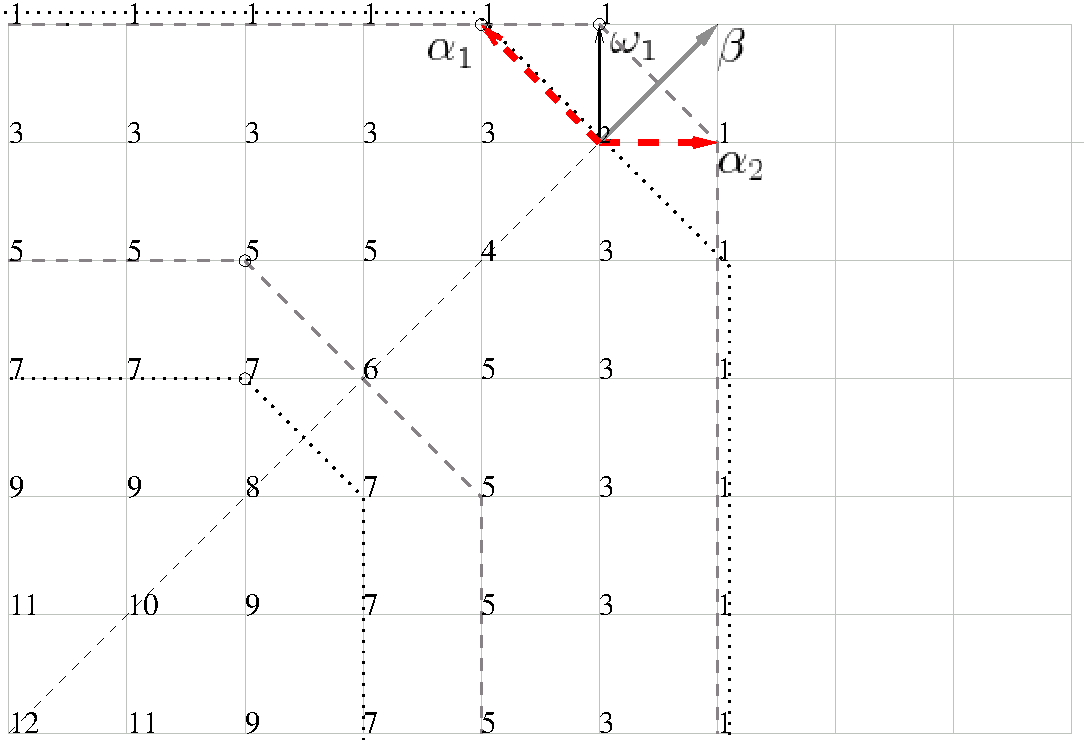
\includegraphics[width=120mm]{B2_Gen_Verma_Decomp}
  }
  \caption{Обобщенные модули Верма для регулярного вложения  $A_1$ в $B_2$. 
    Простые корни $\alpha_1, \alpha_2$ алгебры $B_2$ показаны пунктирными стрелками. Простой корень  $\beta = \alpha_1+2\alpha_2$ алгебры $A_1$ изображен серым вектором. Разложение $L^{\omega_{1}}$ представлено набором контуров входящих в него обобщенных модулей Верма. Пунктирные контуры соответствуют положительным значениям  $\epsilon(u)$, а точечные -- отрицательным. }

 \label{fig:B2_Verma_Decomp}
\end{figure}

\end{example}

\begin{remark}
Как доказано, например, в книге  \cite{humphreys2008representations} (см. утверждение 9.6), характеры обобщенных модулей Верма $M_{I}^{\mu _{\frak{a}_{\perp }}\left( u\right) }$ могут также описываться как линейные комбинации обычных модулей Верма алгебры $\frak{g}$:
\begin{equation*}
\mathrm{ch}M_{I}^{\mu _{\frak{a}_{\perp }}\left( u\right) }=\sum_{w\in W_{%
\frak{a}_{\perp }}}\epsilon \left( w\right) \mathrm{ch}M^{w\left( \mu _{%
\frak{a}_{\perp }}\left( u\right) +\rho _{\frak{a}_{\perp }}\right) -\rho _{%
\frak{a}_{\perp }}}
\end{equation*}
Подставляя это выражение в формулу (\ref{char in gen verma mod}) и используя определения  (\ref{mu-a},\ref{mu-a-tilda}) и (\ref{defect ort}), мы восстанавливаем стандартное разложение Вейля-Верма для характера:
\begin{equation*}
\mathrm{ch}\left( L^{\mu }\right) =\sum_{w\in W}\;\epsilon (u)\mathrm{ch}%
M^{w\left( \mu +\rho \right) -\rho }.
\end{equation*}
\end{remark}

\section{БГГ резольвента и ветвление}
В работе \cite{lepowsky1977generalization} показано, что для модуля старшего веса $L^{\mu }$, где $\mu \in P^{+}$, последовательность (обобщенная БГГ резольвента)
\begin{equation}
0\rightarrow M_{r}^{I}\overset{\delta _{r}}{\rightarrow }M_{r-1}^{I}\overset{%
\delta _{r-1}}{\rightarrow }\ldots \overset{\delta _{1}}{\rightarrow }%
M_{0}^{I}\overset{\varepsilon }{\rightarrow }L^{\mu }\rightarrow 0,
\label{resolution sequence}
\end{equation}
где
\begin{equation}
M_{k}^{I}=\bigoplus_{u\in U,\;\mathrm{length}\left( u\right)
=k}M_{I}^{u\left( \mu +\rho \right) -\rho },\quad M_{0}^{I}=M_{I}^{\mu }
\label{Verma elements sequence}
\end{equation}
является точной и формула (\ref{gen Weyl-Verma}%
) следует из этого разложения.

\begin{figure}[h!bt]
 \noindent\centering{
   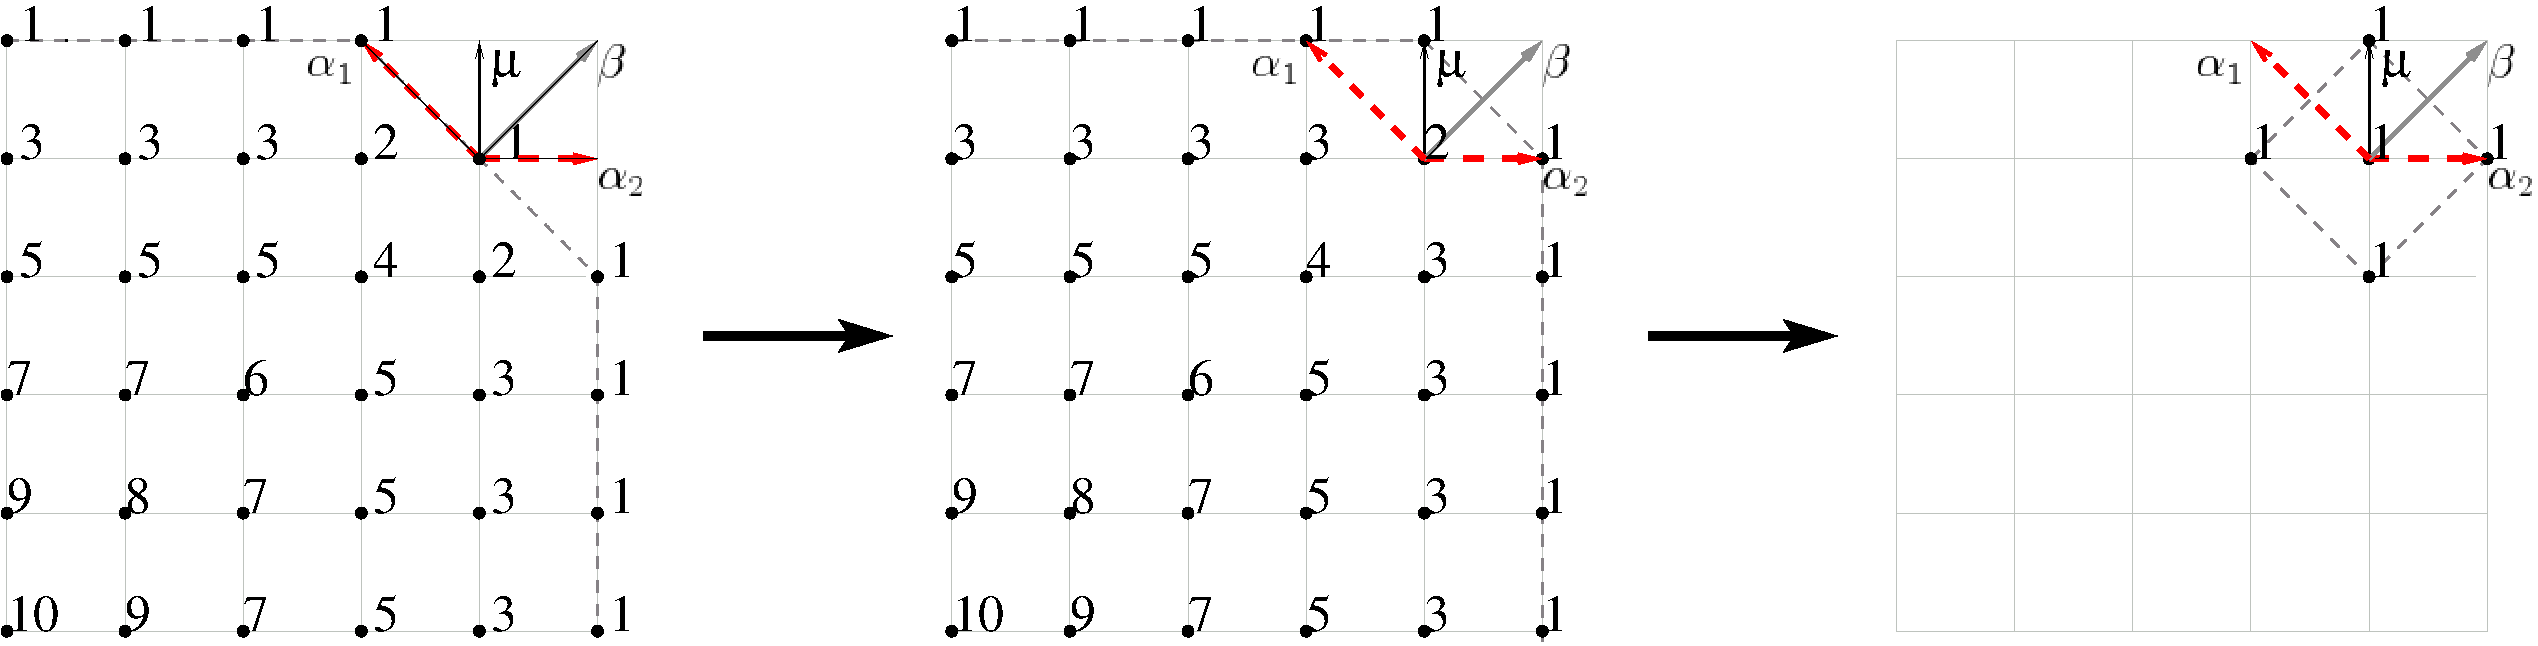
\includegraphics[width=140mm]{B2_Exact}}
 \caption{Вложение $A_1\hookrightarrow B_2$ (см. Рисунок \ref{fig:B2_Verma_Decomp}). Ортогональный партнер, подалгебра $A_1$, соответствует корню $\alpha_1$.
   Резольвента простого модуля $L^{\omega_1}$. Показана центральная часть точной последовательности
   $0 \to Im(\delta_2) \to \left( e^{\mu _{\widetilde{%
\frak{a}}}\left( e\right) }\mathrm{ch}M_{I}^{\pi _{\afb}\left[ \omega_1 \right] -%
\mathcal{D}_{\afb} }=M^{\omega_1}_{I}\right) \to
   L^{\omega_1}\to 0 $.  Здесь $\mu _{\widetilde{\frak{a}}}\left( e\right) =\pi _{\aft}\left[ \mu \right] + \mathcal{D}_{\afb}$.
   }
\end{figure}


\begin{statement}
Пусть $L^{\mu }$ --  $\frak{g}$-модуль со старшим весом $\mu \in P^{+}$, и пусть регулярная подалгебра  $\afb\hookrightarrow \frak{g}$ ортогональна редуктивной подалгебре $\frak{a}\hookrightarrow \frak{g}$. Тогда разложение (\ref{sing decomp main}) определяет как обобщенную резольвенту $L^{\mu }$ по отношению к $\afb$, так и правила ветвления $L^{\mu }$ по отношению к $\frak{a}_{\perp }$, так и правила ветвления $L^{\mu }$ по отношению к подалгебре $\frak{a}_{\perp }$, так и правила ветвления $L^{\mu }$ по отношению к $\frak{a}$ .
\end{statement}

\begin{proof}
Положим
\begin{equation*}
\mathrm{ch}M_{I}^{u\left( \mu +\rho \right) -\rho }=e^{\mu _{\widetilde{%
\frak{a}}}\left( u\right) }\mathrm{ch}M_{I}^{\mu _{\frak{a}_{\perp }}\left(
u\right) },\mathrm{ch}M_{I}^{\mu }=e^{\mu _{\widetilde{\frak{a}}}\left(
e\right) }\mathrm{ch}M_{I}^{\pi _{\frak{a}_{\perp }}\left[ \mu \right] -%
\mathcal{D}_{\frak{a}_{\perp }}},
\end{equation*}
где \ $\mu _{\widetilde{\frak{a}}}\left( u\right) ,\mu _{\frak{a}_{\perp
}}\left( u\right) $ и $\mathcal{D}_{\frak{a}_{\perp }}$ заданы как в Лемме \ref{Psi-decomp-lemma}, $%
u\in U$ определено формулой (\ref{U-def}). В результате получим элементы фильтрующей последовательности (\ref{resolution sequence}).

Рассмотрим множество $\left\{ \mu _{\frak{a}_{\perp }}\left( u\right) |u\in U\right\} $ как множество старших весов простых модулей $L_{\frak{a}%
_{\perp }}^{\mu _{\frak{a}_{\perp }}\left( u\right) }$ и вычислим размерности этих модулей. Вместе с 
$\left\{ \mu _{\widetilde{\mathfrak{a}}}\left( u\right) |u\in
U\right\} $ мы получим набор сингулярных весов
\begin{equation*}
\left\{ \epsilon (u)\;
e^{\mu _{\widetilde{\mathfrak{a}}}\left( u\right) }
\dim \left( L_{\frak{a}_{\perp }}^{\mu _{\frak{a}_{\perp
}}\left( u\right) }\right) \right\} .
\end{equation*}
Ветвление  $L_{\frak{g}\downarrow \frak{a}}^{\mu }=\bigoplus\limits_{\nu
\in P_{\frak{a}}^{+}}b_{\nu }^{\left( \mu \right) }L_{\frak{a}}^{\nu }$  определяется веером вложения  $\Gamma _{\frak{a}\rightarrow \frak{g}}$ и соотношением (\ref{recurrent rel}), которое дает нам коэффициенты  $k_{\xi
}^{\left( \mu \right) }$, а значит определяет и  $b_{\nu }^{\left( \mu \right) }$, так как  $b_{\nu }^{\left( \mu \right) }=k_{\nu }^{\left( \mu
\right) }$ при $\nu \in \overline{C_{\frak{a}}}$ .
\end{proof}

\begin{corollary}
Пусть  $L^{\mu }$ --  $\frak{g}$-модуль со старшим весом $\mu \in P^{+}$ и  $\frak{a}\hookrightarrow \frak{g}$ -- редуктивная подалгебра $\frak{g}$. Пусть $\frak{a}_{\perp }$, ортогональный партнер для $\frak{a}$, эквивалентен  $A_{1}$, $\frak{a}_{\perp }\approx $ $A_{1}$, и $\widetilde{\frak{a}}=\frak{a}\oplus \frak{h}_{\perp }$ с $\frak{h=\frak{h}_{\frak{a}}}\oplus \frak{h}_{\frak{a}_{\perp }}\oplus \frak{h}_{\perp }$. Пусть $L_{\frak{g}\downarrow \widetilde{\frak{a}}}^{\mu }=\bigoplus\limits_{\nu \in P_{\widetilde{\frak{a}}}^{+}}b_{\nu }^{\left( \mu \right) }L_{\widetilde{\frak{a}}}^{\nu }$ -- ветвление модуля $L^{\mu }$ относительно подалгебры $\widetilde{\frak{%
a}}$. Тогда коэффициенты $b_{\nu }^{\left( \mu \right) }$ определяют обобщенную резольвенту (\ref{resolution sequence}) модуля $L^{\mu }$
по отношению к  $\frak{a}_{\perp }$.
\end{corollary}

\begin{proof}
Пусть $\alpha $ -- простой корень  $A_{1}$. Используем преобразования из группы Вейля чтобы перевести его в некоторый простой корень алгебры $\frak{g}$, например $\alpha _{1}$. Построим сингулярный элемент для модуля  $L_{\frak{g}\downarrow
\widetilde{\frak{a}}}^{\mu }$, то есть  $\Psi _{\widetilde{\frak{a}}%
}^{\left( L_{\frak{g}\downarrow \widetilde{\frak{a}}}^{\mu }\right)
}=\sum_{\nu \in P_{\widetilde{\frak{a}}}^{+},b_{\nu }^{\left( \mu \right)
}>0}b_{\nu }^{\left( \mu \right) }\Psi _{\widetilde{\frak{a}}}^{\left( \nu
\right) }$, и разложим его $\Psi _{\widetilde{\frak{a}}}^{\left( L_{\frak{%
g}\downarrow \widetilde{\frak{a}}}^{\mu }\right) }=k_{\xi }^{\left( \mu
\right) }e^{\xi }$. В нашем случае представители $u$ в рекуррентном соотношении (\ref{recurrent rel}) определяются весом $\xi $ однозначно:
\begin{equation*}
\epsilon (u\left( \xi \right) )\;\dim \left( L_{\frak{a}_{\perp }}^{\mu _{%
\frak{a}_{\perp }}\left( u\left( \xi \right) \right) }\right) =-s\left(
\gamma _{0}\right) k_{\xi }^{\left( \mu \right) }-\sum_{\gamma \in \Gamma _{%
\widetilde{\frak{a}}\rightarrow \frak{g}}}s\left( \gamma +\gamma _{0}\right)
k_{\xi +\gamma }^{\left( \mu \right) }.
\end{equation*}
Тогда
\begin{equation*}
\dim \left( L_{\frak{a}_{\perp }}^{\mu _{\frak{a}_{\perp }}\left( u\left(
\xi \right) \right) }\right) =\left| s\left( \gamma _{0}\right) k_{\xi
}^{\left( \mu \right) }+\sum_{\gamma \in \Gamma _{\widetilde{\frak{a}}%
\rightarrow \frak{g}}}s\left( \gamma +\gamma _{0}\right) k_{\xi +\gamma
}^{\left( \mu \right) }\right|
\end{equation*}
и
\begin{equation*}
\mu _{\frak{a}_{\perp }}\left( u\left( \xi \right) \right) =\frac{1}{2}%
\left( \dim \left( L_{A_{1}}^{\mu \left( \xi \right) }\right) -1\right)
\alpha _{1}
\end{equation*}
Таким образом, множество обобщенных модулей Верма  $e^{\xi +\mathcal{D}%
_{\frak{a}_{\perp }}}\mathrm{ch}M_{I}^{\mu _{\frak{a}_{\perp }}\left(
u\left( \xi \right) \right) }$ полностью фиксировано:
\begin{equation*}
\left\{ e^{\mu _{\widetilde{\mathfrak{a}}}\left( u\right) }\mathrm{ch}%
M_{I}^{\mu _{\frak{a}_{\perp }}\left( u\right) }|u\in U\right\} .
\end{equation*}
Упорядочивая эти модули по длине $u$, мы получаем компоненты (\ref{Verma elements sequence}) резольвенты (\ref{resolution sequence}).
\end{proof}



\section{Выводы к третьей главе}

\label{sec:conclusions}
В главе \ref{cha:affine-lie-algebras}  было показано, что метод веера вложения работает также и для специальных вложений. Надо заметить, что  разложения Вейля-Верма также могут быть получены в этом случае. Резольвенты, соответствующие специальным подалгебрам, описывают соотношения между проекциями характера начального модуля и обобщенными модулями Верма со старшими весами в подпространстве $h^*$.

Рассмотрим ситуацию, когда выбор простых корней зафиксирован какими-то внешними факторами (возникающими, например, из требований физических приложений). В этом случае ортогональный партнер не может порождаться только простыми корнями. Элементы   $\frak{u}_{I}^{+}:=\sum_{\eta \in \Delta
^{+}\setminus \Delta _{I}^{+}}\frak{g}_{\eta }$ не образуют подалгебру в  $%
\mathfrak{g}$, так как некоторые не простые корни отсутствуют в  $\Delta ^{+}\setminus
\Delta _{I}^{+}$. Важно отметить, что в этом случае формула Вейля-Верма по-прежнему существует. В ней обобщенные модули Верма соответствуют сжатиями \cite{Doebner1967Melsheimer} алгебры $%
\frak{n}^{+}$ и соотношения Вейля-Верма описывают разложение пространства представления $L^{\mu}$ в набор обобщенных модулей Верма сжатой алгебры  $U\left(\frak{n}_c^{+}\right)$. Весовые векторы образованы базисом Пуанкаре-Биркгофа-Витта алгебр $U\left(\frak{n}_c^{+}\right)$ и
$U\left( \mathfrak{a}_{\bot} \right)$. Чтобы рассмотреть такое пространство как  $%
\mathfrak{g}$-модуль мы должны выполнить деформацию \cite
{Nijenhuis1966Richardson} алгебры $\frak{n}_c^{+}$ (то есть восстановить первоначальный закон композиции). Пространство сохраняется, и после такой деформации генераторы начальной алгебры будут действовать на нем правильным образом.



%%
%% End of file
%%% Local Variables: 
%%% mode: latex
%%% TeX-master: "thesis"
%%% End: 
